\chapter{Introduction}\label{ch:intro}

\section{Context}\label{sec:intro-context}

% historical context
As of 2022 most of the industrialized world has developed tools for unprecedented growth in wealth and technology on a global scale~\cite[Chapter 4]{technology-and-inequalities}. In such times a great deal of consumerism and interconnection is present with people needing products produced faster and more consistently than ever before~\cite[Chapter 4]{technology-and-inequalities}. 
As one would expect, this creates a high demand for manufacturers to reliably and consistently provide products, while also remaining flexible as the demand for different product change rapidly. 
% argue for why automation is better
To accommodate the need for ever-greater volumes of products, consistent, reliable and flexible labor is essential in assembly, transport and manipulation processes in the production pipeline. Due to these types of manual labor being largely done by unskilled workers, automation alternatives are being adopted which provide benefits~\cite[Chapter 4]{technology-and-inequalities}. This different approach to manufacturing has been labeled the fourth industrial revolution or i4.0 for short.
% benefits for the employer
The beneficiaries are the employer and employee, with the employer having the benefits: Avoid paying monthly salaries to unskilled laborers doing manual tasks, here the automation alternative only requires electrical energy and potential supervision by a few qualified individuals. Potential risks are also involved when hiring humans as the workforce can be inconsistent due to human error~\cite{analysis-and-control-of-human-error} or left out due to illness etc. Considerations about workers' rights such as working conditions and wages also need not be considered. Workers furthermore cause production limitations in the form of stand-still hours, such as bathroom and lunch breaks along with after-work hours and holidays.
% benefits for the employee 
This replacement of manual labor also potentially benefits the employee, as boring and physically wearing work is automated, enabling the employees to take on different and less wearing and potentially dangerous roles. While the issue of labor unemployment becomes apparent solutions that provide support to already hired workers have been developed, such as \gls{cobot}~\cite{cobots-and-the-benefits-of-their-implementation-in-intelligent-manufacturing} which would negate this problem. \medskip

% categories of problems in robotics for factories
When implementing automation of production lines using robotics, certain categories of problems are revealed. These include assembly, alteration and \gls{pnp}, the last being the one of interest in this project. 

\section{Problem Description}\label{sec:intro-problem-description}
% applications
Pick-and-place \gls{manipulator}s are used in a wide variety of different fields such as 
sorting of waste~\cite{robotic-pick-and-toss-facilitates-urban-waste-sorting}
handling of food~\cite{automation-of-mobile-pick-and-place-robotic-system-for-small-food-industry, development-of-a-food-handling-soft-robot-hand-considering-a-high-speed-pick-and-place-task} and factory bin picking~\cite{real-time-industrial-bin-picking-with-a-hybrid-deep-learning-engineering-approach, a-bin-picking-benchmark-for-systematic-evaluation-of-robotic-pick-and-place-systems, generic-development-of-bin-pick-and-place-system-based-on-robot-operating-system}. The solutions in these industries are examples of subcategories under the \gls{pnp} problem, namely sorting and bin picking. Since both of these are subcategories of the \gls{pnp} problem, they fundamentally follow the same sequential four phases from start to end. 
% All of these problems fundamentally contain the same structure as shared among all pick-and-place problems.
These phases are pre-grasping, grasping, transport, and placement~\cite{a-bin-picking-benchmark-for-systematic-evaluation-of-robotic-pick-and-place-systems} for traditional implementations of the \gls{pnp} pipeline.
% pre-grasp
The pre-grasp phase involves localizing the object(s), potentially estimating their pose and executing the trajectory to move the \gls{ee} grasp, collision-free to said object(s). Here different potential grasps can be considered to determine the best pose for the \gls{ee}.
% grasping
In the grasping phase, the \gls{ee} gasps the object in such a manner that the object's entire weight is supported by the \gls{ee}, and ends when the object no longer is in contact with the environment, which often is the container holding the object.
% transport
The transportation phase involves the motion of the \gls{manipulator} to move from the pose achieved after the grasping phase, to a pose ready for placement of the object in the desired placing area or fixture. Here considerations may be needed about how much force and torque the \gls{ee}'s grasp can tolerate while moving without losing the object.
% placement
Finally, the goal of the placing phase is to place the object within the placing area or fixture in a desired end pose. Here the constraints on the end pose might differ significantly based on the application, as the pose of greens in a crate might need less precision than if the manipulator hands a bolt to another robotics system in the pipeline. \medskip

While these phases make up a traditional \gls{pnp} system, certain assumptions are made regarding the objects of interest for this pipeline to function. Specifically, the localization and \gls{pe} of the pre-grasp phase are assumed possible due to either ensured object poses or estimated poses through \gls{cv} sensory system. Due to \gls{cv} being a mature research field a wide range of solution proposals to these problems have been generated~\cite{6d-pose-estimation-of-objects:-recent-technologies-and-challenges}. These include classic vision~\cite{3d-object-pose-estimation-using-stereo-vision-for-object-manipulation-system, stereo-vision-based-automation-for-a-bin-picking-solution}, \gls{dl} based~\cite{uncalibrated-stereo-vision-with-deep-learning-for-6-dof-pose-estimation-for-a-robot-arm-system} and combinations of these~\cite{stereo-vision-based-single-shot-6d-object-pose-estimation-for-bin-picking-by-a-robot-manipulator}. However, while these may be sufficient for certain tasks they fundamentally suffer from the weaknesses introduced by vision techniques. These are a great number of outliers caused by: occlusions, reflecting, transparent or homogeneous surfaces, and repetitive structures when solving the \gls{corr-problem}. Within factory settings, the common ones are transparent and reflective objects, due to metallic, plastic and glass products often being the materials used. While \gls{dl} solutions have been developed for both reflective~\cite{data-driven-object-pose-estimation-in-a-practical-bin-picking-application} and transparent~\cite{6dof-pose-estimation-of-transparent-object-from-a-single-rgb-d-image} objects, these are use case specific and show limited results in a wider range of applications. \medskip

This project suggests a different \gls{pnp} pipeline for cases where the object's starting pose is unknown. In this \gls{pnp} pipeline the \gls{pe} is moved from the pre-grasping phase to a new phase between the grasping and transportation phase, called the \gls{pe} phase. The specific goal of this project is to develop a solution to this phase using tactile sensors in the \gls{ee} to determine the object's pose. By using tactile sensing rather than visual the problems presented above will be eliminated. This will be done using a humanoid gripper as the \gls{ee} with tactile sensors in each finger, more specifically a Shadow Dexterous Hand~\cite{shadow-dex-hand} with \num{20} \gls{dof}. \medskip
% pre-grasping, grasping, transport, and placement

The alternative pipeline this project will enable can be seen in the upper row of \figref{fig:pnp-pipeline} compared to the traditional pipeline in the lower row.\medskip 

% pre-grasping phase
In \figref{fig:pre-grasp-phase} the pre-grasping phase can be seen for both pipelines. Here the traditional pipeline in cases of multiple objects often will employ custom fingertips or grippers entirely to facilitate form closure grasps, due to the grippers not having the flexibility to perform reliable force closure. On the contrary force closure can be performed with a humanoid gripper on a wide range of objects with no need for changing gripper equipment. \medskip

% grasping phase
In \figref{fig:grasping-phase} the grasping phase can be seen which introduces a greater level of complexity when using the suggested pipeline due to the humanoid gripper being a more complex physical system to represent and control. This is compared to the simplicity of executing potential binary commands in the traditional pipeline e.g.open and close. \medskip

% transportation phase
In \figref{fig:transportation-phase} the transportation phase can be seen, which introduces one of the benefits of using the suggested pipeline. Here tactile sensors in a humanoid gripper can pose and estimate the object and manipulations can be performed to change the object's pose such that easier placement can be performed in the following phase. This form of object manipulation is not feasible for the simple pneumatic grippers used in a traditional pipeline. \medskip

% placement
In \figref{fig:placement-phase} the placement phase can be seen, which demonstrates the result of the previous phase, as the traditional pipeline now has to change the grip on the object to properly place it in the socket, while the humanoid gripper simply can insert the part, as it is already oriented properly. \medskip

\newpage

\begin{figure}[h]
	\centering
	\begin{subfigure}[b]{0.24\textwidth}
		\centering
		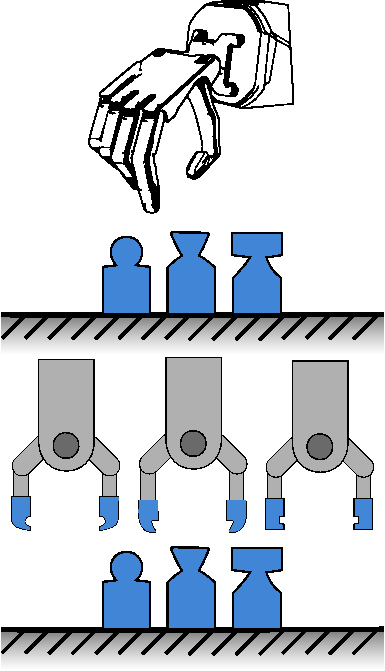
\includegraphics[width=\textwidth]{chapters/introduction/fig/pipeline-1.pdf}
		\caption{Pre-grasp phase.}
		\label{fig:pre-grasp-phase}
	\end{subfigure}
	\hfill
	\begin{subfigure}[b]{0.24\textwidth}
		\centering
		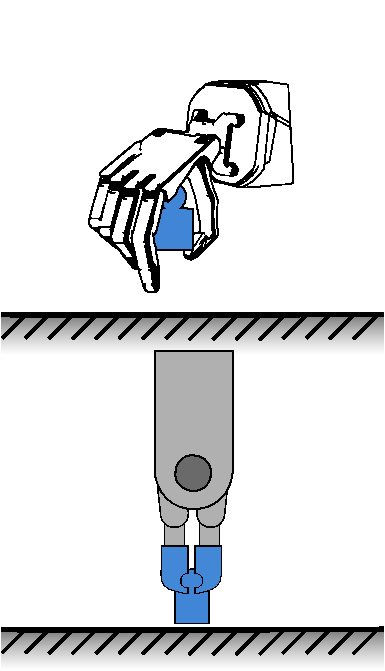
\includegraphics[width=\textwidth]{chapters/introduction/fig/pipeline-2.pdf}
		\caption{Grasping phase.}
		\label{fig:grasping-phase}
	\end{subfigure}
	\hfill
	\begin{subfigure}[b]{0.24\textwidth}
		\centering
		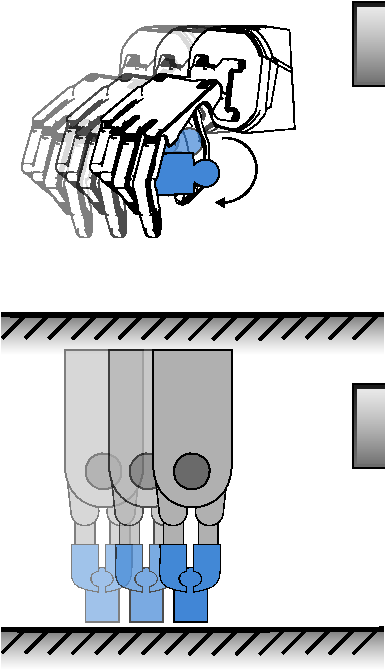
\includegraphics[width=\textwidth]{chapters/introduction/fig/pipeline-3.pdf}
		\caption{Transportation phase.}
		\label{fig:transportation-phase}
	\end{subfigure}
	\hfill
	\begin{subfigure}[b]{0.24\textwidth}
		\centering
		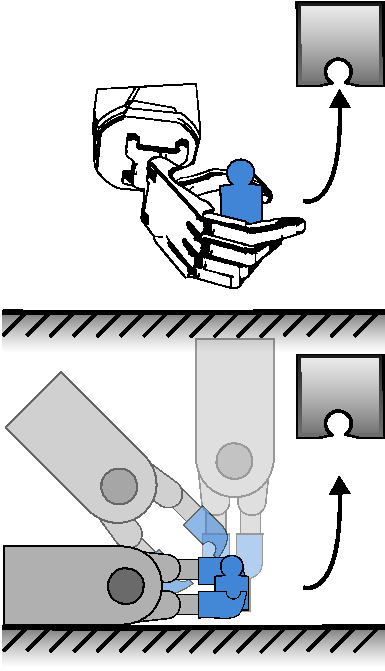
\includegraphics[width=\textwidth]{chapters/introduction/fig/pipeline-4.pdf}
		\caption{Placement phase.}
		\label{fig:placement-phase}
	\end{subfigure}
		\caption{A comparison between the traditional and suggested \gls{pnp} pipeline.}
		\label{fig:pnp-pipeline}
\end{figure}


To solve this \gls{pe} problem, three sub-problems are identified and labeled problems \num{1}, \num{2} and \num{3}.
% problem 1
\begin{problem} \label{prob:1}
	\normalfont involves modeling the contact between the gripper's tactile sensors and the object, also referred to as tactile perception. 
\end{problem}

% problem 2
\begin{problem} \label{prob:2}
	\normalfont is to convert the collected data from problem 1 to estimated pose candidates.
\end{problem}

% problem 3
\begin{problem} \label{prob:3}
	\normalfont involves in-hand manipulation. Since the initial grasp of the object might not be oriented in a manner where the recognizable features make context with the tactile sensors, manipulating the object within the \gls{ee}'s grasp will enable further information gathering. Thus the final problem is to control the \gls{ee} in such a manner that the tactile sensors make context with the object in intelligently decided areas for a better pose estimate.
\end{problem}

To test if the developed system successfully solves the \gls{pe} problem, it is hypothesized that the intelligent probing method provides a statistically significant faster average \gls{pe} convergence, along with a statistically significant greater success rate when determining the correct pose. A correct pose is here defined as the pose being greater than or equal to \SI{95}{\percent} of the ground truth pose, and statistically significant is defined by an $\alpha$-level of \SI{95}{\percent}. This hypothesis will be referred to as $\text{H}_1$, while the null hypothesis $\text{H}_0$ being that there is no statistically significant difference between intelligent and random probing's \gls{pe} performance as described above.

% more accurate estimates of the pose and does so in a shorter time span than simply sensing the object's surface in random locations $\text{H}_1$. 
% This is compared to the null hypothesis, that there is no statistically significant difference in the methods' \gls{pe} performance $\text{H}_0$.

% such that further information is gained by probing the object. Here new desired surface points are found through intelligent probing such that strong surface features are found to better identify the object's correct pose. \medskip

% A pipeline where the estimation of object poses is moved from the pre-grasping to the grasping phase, where the weaknesses from the current methodology are eliminated. This is achieved by using tactile sensors, thus eliminating the need for visual features and as a product also eliminating the problems listed above. 

% Thus, this project suggests a \gls{pnp} pipeline which moves the pose estimation from the pre-grasping phase to a new phase between the grasping and transportation phase. This new phase is called the pose estimation phase. The overarching goal of this project is to develop a solution to the pose estimation phase using tactile sensors in the \gls{ee} to find surface features and use these to determine the object's pose.

% traditional pipeline makes assumptions -> 

% and end effector pose est
\section{Thesis Overview}\label{sec:intro-thesis-overview}

This project is composed of \num{9} chapters, each listed below with an associated description. \medskip

% To present the work done in this project, the system modeling is done in~\chapref{ch:modeling} and \gls{sota} is presented in~\chapref{ch:state-of-the-art} for each of the problems presented above. Here the solutions best suited for this project's gripper are chosen. Each solution is described in detail, how they are applied, their performance tested and finally evaluated and concluded upon in their respective chapters i.e. chapter~\chapref{ch:1-tactile-perception},~\chapref{ch:2-pose-estimation} and~\chapref{ch:3-in-hand-manipulation}. In~\chapref{ch:4-system-integration} the three methods are combined in the final integration and finally, the project is discussed and concluded upon in~\chapref{ch:discussion} and~\chapref{ch:conclusion} respectively.

\textbf{Chapter 1:} The introduction presents the historical context of the project along with a problem description and thesis overview. The problem description contains the decomposition of the project into sub-problems which will be addressed in the following chapters. \medskip

\textbf{Chapter 2:} The system setup presents an overview of the practical details of the project in the form of the system setup along with the code developed to execute the project. \medskip

\textbf{Chapter 3:} The literature review addresses the three problems identified in \chapref{ch:intro} by providing a thorough literature review on older as well as newer methods for solving each of the identified problems. To end each section, groups are compared and a method is chosen among the ones presented. \medskip

\textbf{Chapter 4:} The modeling chapter presents the physical modeling of the system and defines important mathematical notations and quantities as used in the following chapters. \medskip

\textbf{Chapter 5:} The \gls{tp} chapter addresses the method chosen in \chapref{ch:state-of-the-art} to solve the first problem. This chapter expands on the method chosen and its functionality, followed by an evaluation of said method through experiments and their results. Finally, the functionality of the method is concluded. \medskip

\textbf{Chapter 6:} The \gls{pe} chapter addresses the method chosen in \chapref{ch:state-of-the-art} to solve the second problem. This chapter follows the same structure as \chapref{ch:1-tactile-perception}. \medskip

\textbf{Chapter 7:} The \gls{ihm} chapter addresses the method chosen in \chapref{ch:state-of-the-art} to solve the third problem. This chapter follows the same structure as \chapref{ch:1-tactile-perception} and \chapref{ch:2-pose-estimation}. \medskip

\textbf{Chapter 8:} The discussion chapter goes over the combined system and addresses problems, improvements, shortcomings and potential for future development.

\textbf{Chapter 9:} The conclusion chapter addresses the successfulness of the project.

% The developments in robotics as a field have over the past years provided automation solutions to execute repetitive manual tasks with high efficiency and reliability \fakecite. One of the most common tasks is pick and place tasks which involve picking up an object from one position and placing it in another. This is can be parted into the following subparts: Object localization, pose estimation, grasping and placing. In the solutions currently present for industrial use \gls{cv} is used for object localization and \gls{pe} due to the low cost of cameras and the field's maturity. However, while these solutions may be sufficient for certain tasks they fundamentally suffer from the weaknesses introduced by vision techniques. These include a great number of outliers caused by occlusions, reflecting, transparent or homogeneous surfaces, and repetitive structures when solving the \gls{corr-problem}. These problems as of the writing of this project have yet to be completely solved. Promising results have been found with the rise of \gls{dl} which in the present time has proven its versatility and provides proof of concept solutions for narrow cases in pose estimation of transparent \cite{6dof-pose-estimation-of-transparent-object-from-a-single-rgb-d-image} and reflective \medskip

% \begin{minipage}{0.45\textwidth}
% 	objects \cite{6d-pose-estimation-of-objects:-recent-technologies-and-challenges}. This is relevant since industrial settings often contain transparent and especially reflecting objects as metallic parts tend to appear frequently and have high reflectances. To solve these problems this project aims to perform in-hand pose estimation through only the use of tactile sensors. Specifically, this will be done on a Shadow Dexterous Hand \cite{shadow-dex-hand} with 20 \gls{dof}. Using tactile inputs rather than visual eliminates the weaknesses mentioned above. A schematic showing the hand can be seen in \figref{fig:shadow-dex-hand-schematic}. Using this approach, the overall problem can be partitioned into 3 sub-problems labeled problems 1, 2 and 3. Problem 1 involves modeling the contact between the gripper's fingers and the object, also referred to as tactile perception. Problem 2 is to convert the collected data from problem 1 to meaningful surface data, treat these data as features and use them to estimate pose candidates. Finally, problem 3 involves in-hand manipulation, such that further information is gained by probing the object. Here new desired surface points are found through intelligent probing such that strong surface features are found to better identify the object's correct pose. \medskip
% 	\end{minipage} 
% 	\hfill
% 	\begin{minipage}{0.45\textwidth}
% 	\begin{figure}[H]
% 		\begin{small}
% 			\begin{center}
% 				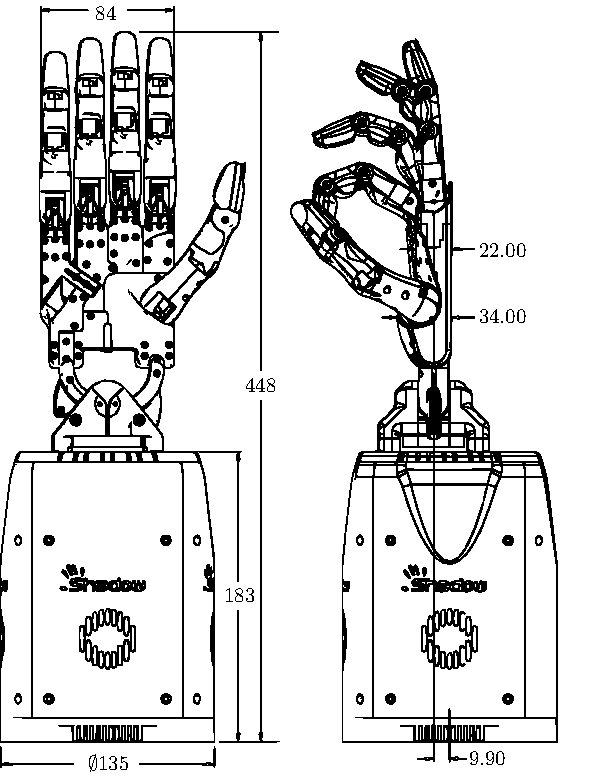
\includegraphics[width=0.95\textwidth]{chapters/introduction/fig/shadow-dex-hand-vector.pdf}
% 			\end{center}
% 			\caption{Schematic of Shadow Dexterous Hand from Shadow Robots, based on \cite{shadow-dex-hand-schematic}. The measurements are in \SI{}{\milli\metre}.}
% 			\label{fig:shadow-dex-hand-schematic}
% 		\end{small}
% 	\end{figure}
% \end{minipage}

% Thus the hypothesis of this projects $\text{H}_1$, will be testing if intelligent probing for strong features increases in-hand pose estimation performance, with the null hypothesis $\text{H}_0$ being that there is no statistically significant difference in the pose estimation performance of the system if the probing is done randomly or intelligently at a certainty level of \highlight{95\%}. Here pose estimation performance is quantified in terms of mean execution time for estimating the pose with an accuracy greater than \highlight{95\%}. \medskip

% The development of this project is done in the \gls{docker} provided by Shadow Robotics for simulation, control and development of the hand \cite{shadow-dex-github}. Here a hardware-simulation agnostic \gls{ros} \cite{ros} control \cite{ros-control} interface is found, which contains fundamental tools to interact with the robot hand. The dynamic simulation environment Gazebo \cite{gazebo} is likewise packaged as part of the \gls{docker} and is thus the one used for this project.
% To solve the problems presented, the \gls{ros} packages in \tabref{tab:software-package-table} will be applied, where \texttt{ros\_utils} and \texttt{in\_hand\_pose\_estimation} will be developed during this project.

% \begin{table}[h]
% 	\begin{small}
% 		\begin{center}
% 			\begin{tabular}[c]{ | l r | l | } \hline
% 				\cellcolor{tableheader} \textbf{Package}           & \cellcolor{tableheader} & \multicolumn{1}{l|}{\cellcolor{tableheader} \textbf{Description}} \\ \hline \hline
% 				\texttt{in\_hand\_pose\_estimation}                & \meta{meta} & \textbf{Project package of the in-hand pose estimation system} \\ \hline
% 				\hspace{0.3cm} \texttt{in\_hand\_pose\_estimation} &             & Integration of the full in-hand pose estimation pipeline  \\ \hline
% 				\hspace{0.3cm} \texttt{sr\_tactile\_image}         & \pkg{pkg}   & Extraction of tactile perception  \\ \hline
% 				\hspace{0.3cm} \texttt{sr\_pose\_estiamtion}       & \pkg{pkg}   & Estimate the pose of object based on tactile perception \\ \hline
% 				\hspace{0.3cm} \texttt{sr\_hand\_manipulation}     & \pkg{pkg}   & Manipulate object in hand to probe for strong features \\ \hline \hline
% 				\texttt{sr\_common}                                & \meta{meta} & \textbf{Shadow package for commonly used tools} \\ \hline
% 				\hspace{0.3cm} \texttt{sr\_common}                 &             & Implements commonly used tools such as messages \\ \hline
% 				\hspace{0.3cm} \texttt{sr\_robot\_msgs}            & \pkg{pkg}   & Messages used to communicate with the robot hand  \\ \hline 
% 				\hspace{0.3cm} \texttt{\dots}                      &             &  \\ \hline \hline
% 				\texttt{sr\_core}                                  & \meta{meta} & \textbf{Shadow package for core tools} \\ \hline
% 				\hspace{0.3cm} \texttt{sr\_core}                   &             & Implements core features of the hand such as hardware interfacing \\ \hline
% 				\hspace{0.3cm} \texttt{sr\_hand}                   & \pkg{pkg}   & Contains the hand commander for controlling the robot hand  \\ \hline
% 				\hspace{0.3cm} \texttt{\dots}                      &             &  \\ \hline \hline
% 				\texttt{ros\_utils}                                & \pkg{pkg}   & \textbf{Utilities for interfacing ROS/Gazebo/MoveIt/Eigen etc} \\ \hline
% 			\end{tabular}
% 		\end{center}
% 		\caption{Software packages used in the in-hand pose estimation system.}
% 		\label{tab:software-package-table}
% 	\end{small}
% \end{table}

% To present this work, the \gls{sota} solutions to each of the three problems described above will be presented in~\chapref{ch:state-of-the-art}, where the best fitting methods for this use case will be chosen. In \chapref{ch:1-tactile-perception} to \chapref{ch:3-in-hand-manipulation} these solutions will be presented, analyzed, and their performance discussed and concluded upon. In \chapref{ch:4-system-integration} the system integration will be presented and the total performance of the system will be concluded. Finally, in \chapref{ch:discussion} and \chapref{ch:conclusion} the results and methods will be discussed with potential improvement for future iterations and the project til be concluded.